\documentclass{beamer}
\usepackage{etex}
\usetheme{Warsaw}
\usepackage{amssymb, amsmath}
\usepackage[T1]{fontenc}          %% permet d'utiliser les caractères accentués
\usepackage[utf8]{inputenc}     %% adapte le style article aux conventions francophones
\usepackage[frenchb]{babel}
\usepackage{fancyvrb}
\usepackage{graphics}
\usepackage{pstricks,pstricks-add,pst-math,pst-xkey}
\usepackage{multicol}
\usepackage{graphicx}
\usepackage{algorithm}
\usepackage[nottoc,notlof,notlot]{tocbibind}
%Dash lines

\def\lya{Ly-$\alpha$\ }
\def\sqd{$deg^{2}$}
\def\psqd{$obj \cdot deg^{-2}$}

\def\begeq{\begin{equation}}
\def\endeq{\end{equation}}

\title{Fiber assignment for DESI}
\author{Bob Cahn and Louis Garrigue}
\date{June 2015}
\logo{\includegraphics[height=1cm]{python/representant.jpg}}
\begin{document}

  \begin{frame}
\maketitle
\begin{center}
  
\includegraphics[width = 20mm]{figs/logolbnl.png} \hfill
  \includegraphics[width = 20mm]{figs/logodesi.jpg} \hfill
  
\includegraphics[width = 20mm]{figs/logoens.png} 
\end{center}
  \end{frame}

  \begin{frame}
\begin{center}
  \includegraphics[scale=0.11]{python/representant.jpg}
\end{center}
  \end{frame}
% --------- Sommaire ---------
\begin{frame}
  \tableofcontents
\end{frame}      
% ----------------------------
\section{Code}

\begin{frame}\frametitle{Code}
	\begin{itemize}
		\item library of functions which can be easily adapted, with a "main" producing the assignment
		\item well "pipelined", and someone can use or modify it easily
		\item can be found on \href{https://github.com/desihub/fiberassign}{DESI git repository}
		\item create the executable with a "make all" and run it on NERSC with "qsub run"
	\end{itemize}
\end{frame}

\begin{frame}
	\subsection{Input}\frametitle{Input-Output}
	\begin{itemize} 
		\item Parameters : all parameters, including addresses of other input files
		\item Target DB : information, before the study, on all possible targets
		\item Obs DB : database constructed from the ongoing DESI observations after the data has been processed by the Spectroscopic pipeline. This DB has not been designed yet
		\item Survey tiles : file containing the positions of all the tiles to be observed
		\item Fiber positions : locations of the positioners in the focal plane
	\end{itemize} 
\end{frame}

\begin{frame}\frametitle{Output}
	\subsection{Output}
	FITS files
	\begin{itemize} 
		\item fiber
		\item positioner
		\item number of available objects
		\item ID of available objects
		\item objtype: ELG, LRG, QSO, SKY, STDSTAR, GAL, OTHER
		\item targetid
		\item desi target : targeting info
		\item ra, dec
		\item xfocal, yfocal : mm from center in positioner coordinate system
	\end{itemize} 
\end{frame}

\subsection{Source files}
\begin{frame}\frametitle{Source files}
	Source files are file.h and file.cpp and are in this increasing dependency order :
	\begin{itemize}
		\item misc : manipulate lists, tables, pairs, plots, ...
		\item collision : collision checking of positioners
		\item features : carries all parameters
		\item structs : objects, plates, positioners, assignment information
		\item global : main high-level functions and algorithms
		\item main : neat and quickly understandable code that sums up all the steps of the assignment
	\end{itemize}
\end{frame}

\subsection{Mock catalog}
\begin{frame}\frametitle{Objects}
	\begin{table}[H]\centering
		\begin{tabular}{rcccl} \hline
			Kind&Id&Priority&Nobs&Density (\psqd)\\ \hline
			QSO Ly-$\alpha$ & 0 & 1 & 5 & 50\\
			QSO Tracer & 1 & 1 & 1 & 120\\
			LRG & 2 & 3 & 2 & 300\\
			ELG & 3 & 4 & 1 & 2400\\
			Fake QSO & 4 & 1 & 1 & 90\\
			Fake LRG & 5 & 3 & 1 & 50\\
			Standard Star & 6 & 5 & 1 & 140\\
			Sky Fiber & 7 & 6 & 1 & 1400\\ \hline
		\end{tabular}
		\caption{Characteristics of objects samples} 
	\end{table}
\end{frame}

\subsection{Parameters}
\begin{frame}\frametitle{Parameters}
	\begin{itemize}
			\begin{tiny}
			\item input and output directories
			\item Output = true, whether you want to release the output

			\item Randomize = false randomize order of plates in making plans
			\item Pacman = false selects only spectrometers 0, 1, 2, 7, 8, 9 of the pacman
			\item Npass = 5 number of passes
			\item MaxSS = 10 ; MaxSF = 40 number of fibers assigned to SS and SF on a petal
			\item PlateRadius = $1.65^{\circ}$ radius of the plate
			\item InterPlate = 0 minimal number of plates between two observations of the same galaxy
			\item Analysis = 0, tile distance for getting the information from previously observed tiles
			\item InfDens = false, simulate infinite density of SS and SF

			\item TotalArea = 15789.0 \sqd total area of the sky considered
			\item invFibArea = 700 inverse of area in \sqd accessible to a fiber (fiber density for a \sqd)
			\item moduloGal = 1, if 2 for instance, reads only one object over two in galFile
			\item moduloFiber = 1, same for fiber

			\item PatrolRad = 6.0 mm maximum distance between a positioner to a galaxy

			\item Collision = true when we want to allow collisions
			\item Exact = true whether we want exact geometry collision checking (otherwise just circles)
			\item AvCollide = 3.2 mm in case of no exact collision checking
			\item Collide = 1.98 mm, NoCollide = 7 mm, used to optimize collision checking
			\item NeighborRad = 14.0 mm maximum distance to consider that two fibers are neighbors

			\item PlotObsTime, etc, whether we want to plot some information into output files
			\item Verif = false, whether we verificate that the assignment is sane
			\end{tiny}
	\end{itemize}
\end{frame}

\section{Assignment}
\subsection{Rules}
\begin{frame}\frametitle{Rules}
\begin{itemize}
	\item a tile-fiber is only assigned once
	\item no collision between fiber positioners
	\item two observations of a QSO or an LRG can't be separated by less than {\tt InterPlate} plates
	\item in last pass, only ELG, SS and SF are considered
	\item there are 10 and 40 fibers assigned to SS and SF per petal
	\item try to assign a fiber to the highest prioritized object, then to the least observed
	\item between an already observed \lya and an unknown QSO, one chooses the already observed \lya
	\item the same SS or SF can be observed several times
	\item SS has priority over SF
	\item our policy is : while improving the assignment, never unassign an object without reassigning it right then
\end{itemize}
\end{frame}

\begin{frame}\frametitle{Choose by density}
\begin{figure}[H]\begin{center}
	\includegraphics[scale=0.1]{figs/act.eps}
	\caption{Choice by density : A is chosen to observe 1}\label{act}
\end{center}\end{figure}
Doesn't improve the results
\end{frame}

\begin{frame}\frametitle{Assignment plan}
	\begin{itemize}
		\item make a plan before begining the study, without SS nor SF
		\item begining the real 5-years observation, assigning SS and SF just before observing a tile
		\item update this plan during observations, from information from analysis of exact kinds of objects
	\end{itemize}
\end{frame}


\subsection{First assignment}
\begin{frame}\frametitle{First assignment plan}
	For all plates (tiles) :
	\begin{itemize}
		\item assign QSO
		\item assign LRG
		\item assign ELG
	\end{itemize}
\end{frame}


\subsection{Improve}
\begin{frame}\frametitle{Improvement functions ideas}
	\begin{center}
		\begin{figure}[H]
			\includegraphics[scale=0.7]{figs/graph/idea.pdf}
			\hspace*{1cm}
			\includegraphics[scale=0.7]{figs/graph/transf.pdf}\hfill
			\caption{Improve}\label{transf}
		\end{figure}

		\begin{figure}[H]
			\includegraphics[scale=0.7]{figs/graph/idea1.pdf}
			\hspace*{1cm}
			\includegraphics[scale=0.7]{figs/graph/transf1.pdf}\hfill
			\caption{Redistribute}\label{transf1}
		\end{figure}

		\begin{figure}[H]
			\includegraphics[scale=0.7]{figs/graph/idea2.pdf}
			\hspace*{1cm}
			\includegraphics[scale=0.7]{figs/graph/transf2.pdf}\hfill
			\caption{Improve from kind}\label{transf2}
		\end{figure}
	\end{center}
\end{frame}


\begin{frame}\frametitle{Improving the plan}
	\begin{itemize}
		\item Run, globally, on the list plates from 0 to last :
		\item Simply assign fibers
		\item Redistribute (several times)
		\item Improve + 2x Redistribute (several times)
		\item Redistribute (several times)
	\end{itemize}
\end{frame}


\begin{frame}\frametitle{Improving the plan}
	\begin{figure}[H]
		\hspace*{-0.5cm}
		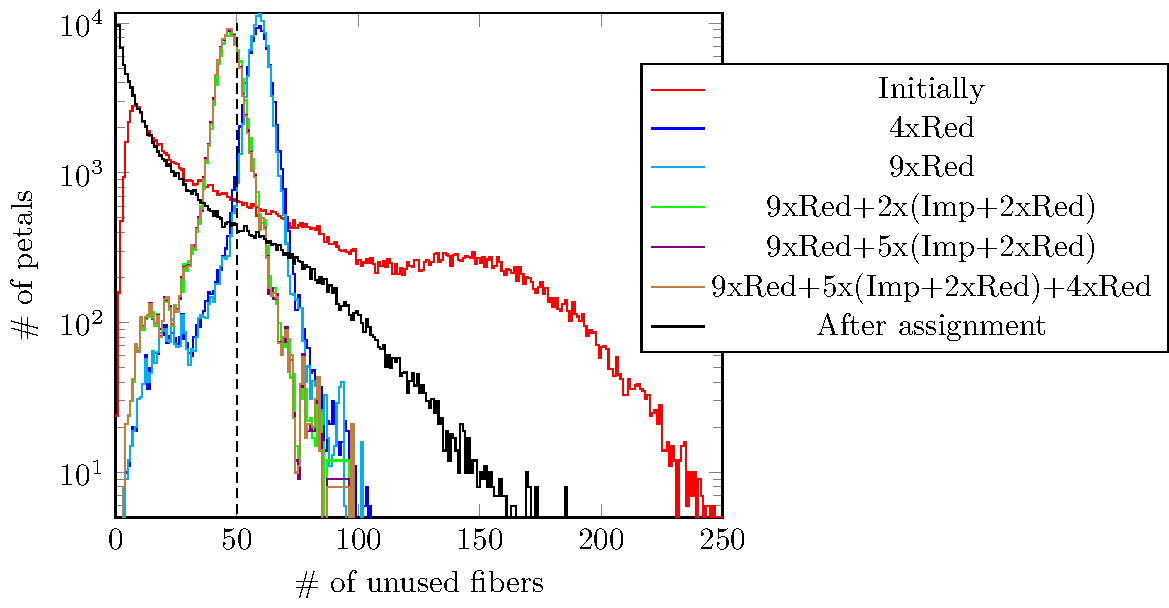
\includegraphics[scale=0.6]{figs/graph/unusedfibs.pdf}
	\end{figure}
\end{frame}


\subsection{Applying the plan}
\begin{frame}\frametitle{Applying the plan}
	Tile after tile, as we observe :
	\begin{itemize}
		\item Assign SS and SF, replacing some ELG
		\item Assign further observed objects to unused fibers if possible
		\item Observe the tile
		\item Update the plan left with information from analysis of previously observed galaxies
		\item Improve the plan left (several redistribute, improve, redistribute)
	\end{itemize}
\end{frame}

\begin{frame}\frametitle{Execution}
\begin{tiny}
\# Read 71,998,144 galaxies from objects\_ss\_sf0.rdzipn \\
\# Read 10,666 plate centers from desi-tiles.par and 5000 fibers from fiberpos.txt \\
\# Start building HTM tree at 13.8 s ... took : 25.5 s \\
\# Begin collecting available galaxies ... took : 31.6 s \\
\# Begin computing available tilefibers ... took : 1 mn 12.5 s \\
\# Start assignment at :  2 mn 27 s \\
\# Begin new assignment : \\
  50,518,743 assignments on all left next plates \\
\# ... took : 18 mn 38.3 s \\
\# Begin improve : \\
  565,801 more assignments (1.120 \% improvement) \\
\# ... took : 36.5 s \\
\# Begin redistribute TF : \\
  1,760,465 redistributions of couples of TF \\
\# ... took : 23.3 s \\
\# Begin real time assignment at 23 mn 24.5 s \\
 - Plate 0 :   550 not as -  3852 unas \& 2772 replaced \\
 - Plate 1 :    98 not as -  3784 unas \& 2773 replaced \\
\# Begin redistribute TF : \\
  1,160,465 redistributions of couples of TF \\
\# ... took : 23.3 s \\
\# Begin improve : \\
  106,948 more assignments (0.205 \% improvement) \\
\# ... took : 30.2 s \\
- Plate 2 :   48 not as -  3128 unas \& 2475 replaced \\
- Plate 3 :    96 not as -  3407 unas \& 2485 replaced \\
\end{tiny}
\end{frame}

\section{Results}
\begin{frame}\frametitle{Results}
\begin{tiny}
\begin{table}[H]\begin{center}
\begin{tabular}{rrrrrrrrrrcc}
\hline
\multicolumn{6}{r}{Times observed} \\
	~ &           0 &     1 &  2 & 3 & 4 & 5 &  Total & Fibused & obs $\%$ & weighted $\%$ \\ \hline
    QSOLy-a   &     0 &     1 &   5 & 12 & 19 & 10 &    49 &   180 &    99.151 & 72.206 \\ 
  QSOTracer   &     1 &   118 &   0 &  0 &  0 &  0 &   119 &   118 &   99.141 & 99.141 \\ 
        LRG   &    13 &    42 & 243 &  0 &  0 &  0 &   298 &   528 &   95.505 & 88.434 \\ 
        ELG   &   480 & 1,930 &   0 &  0 &  0 &  0 & 2,411 & 1,930 & 80.054 & 80.054 \\ 
    FakeQSO   &     0 &    89 &   0 &  0 &  0 &  0 &    90 &    89 &    99.139 & 99.139 \\ 
    FakeLRG   &     2 &    47 &   0 &  0 &  0 &  0 &    50 &    47 &    95.792 & 95.792 \\ 
\hline
\end{tabular}
\caption{Densities (objects/\sqd) as as a function of \# of observations (with total), and \% observed, once and weighted}\label{res}
\end{center}\end{table}
\end{tiny}
51,044,452 assignments in total (95.7143 \% of all fibers)
\end{frame}


\begin{frame}
	\begin{figure}[H]
		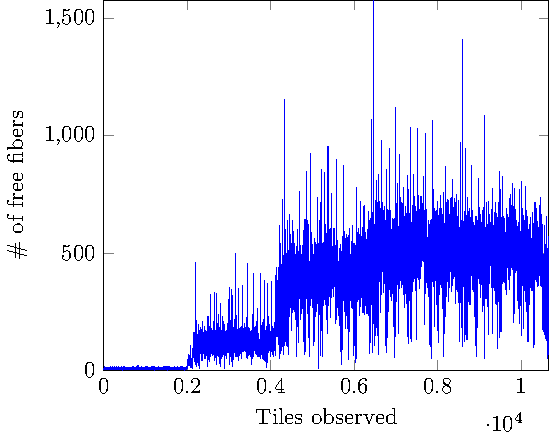
\includegraphics[scale=0.8]{figs/graph/fft.pdf}
		\caption{\# free fibers as a function of time (plates)}\label{fft}
	\end{figure}
\end{frame}


\begin{frame}
\begin{figure}[H]\begin{center}
	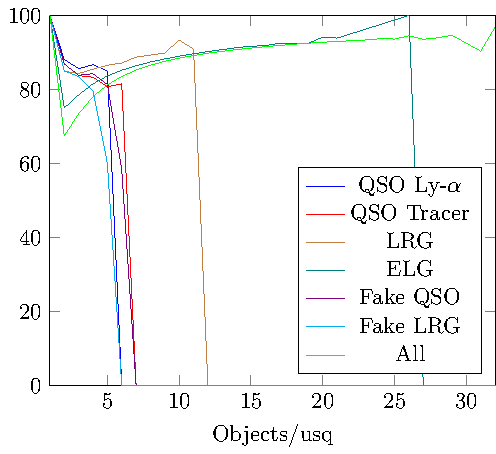
\includegraphics[scale=0.8]{figs/graph/seendens.pdf}
	\caption{\% of observed galaxies as a function of objects density}\label{seendens}
\end{center}\end{figure}
\end{frame}


\begin{frame}
\begin{figure}[H]\begin{center}
	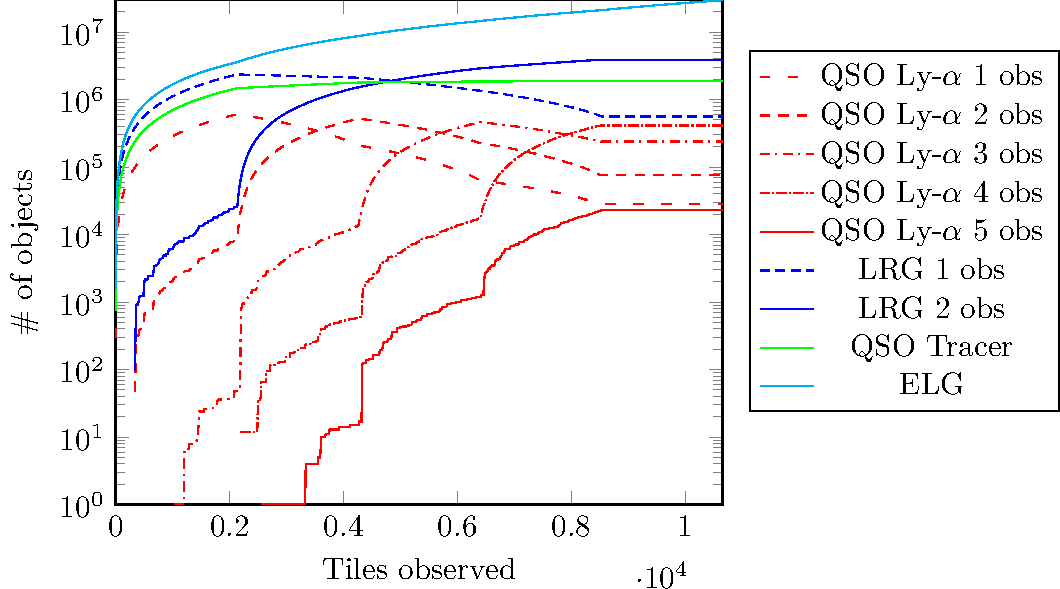
\includegraphics[scale=0.6]{figs/graph/time2.pdf}
	\caption{Observed galaxy kind as a function of time (plates seen)}
\end{center}\end{figure}
\end{frame}





\section{Collision problem}
\begin{frame}\frametitle{Geometry}
\begin{figure}[H]\begin{center}
	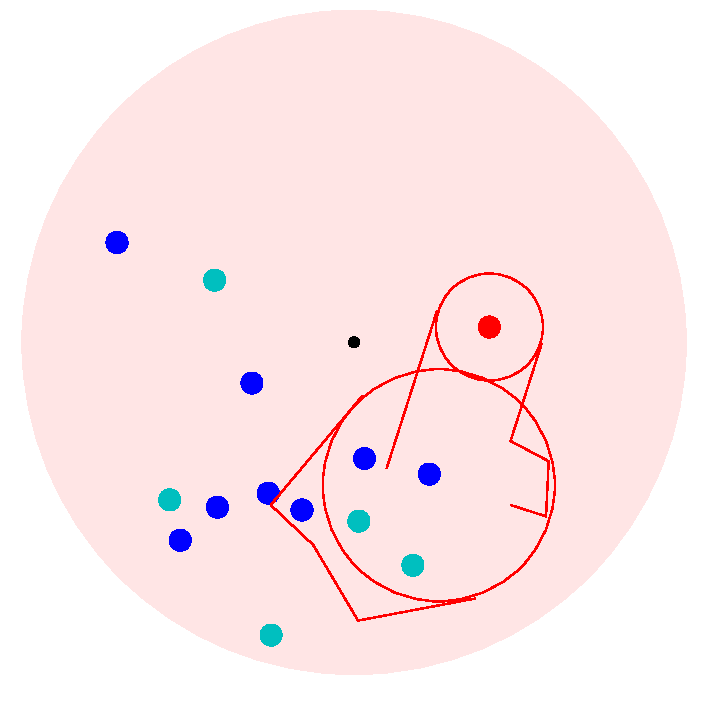
\includegraphics[scale=0.5]{figs/one_fib.pdf}
	\caption{Geometry of a positioner, with fiber holder and central body oriented}\label{onefib}
\end{center}\end{figure}
\end{frame}

\begin{frame}\frametitle{Collision rate}
\begin{figure}[H]\begin{center}
	\includegraphics[scale=0.6]{figs/graph/coldist.pdf}
	\includegraphics[scale=0.6]{figs/graph/coldistint.pdf}
	\caption{Histogram of distances between galaxies in collision cases, and integral}\label{coldist}
\end{center}\end{figure}
Collision rate : 10.8\%
\end{frame}


\section{Conclusion}
\subsection{Optimum}
\begin{frame}\frametitle{Mathematical optimum}
Have we reached the optimum ? Mathematical expressions will give the answer

Imagine a portion S of the sky of the size the reacheable area by a single fiber

Let i be the indice for different kinds (\lya, fake QSO, ... except SS or SF)

Let $\lambda_{i}$ be the densities of the kinds of objects in S

Let N be the indice for the portions of sky with exactly N objects (when we take an area of size S)

Let $f_{k}$ be the fraction of the sky which density corresponds to N

Let $poisson(x,n) = \frac{x^{n}e^{-x}}{n!}$ be the Poisson distribution

Then, for a given ELG in S, named e, the probability to be observed is :
\end{frame}

\begin{frame}
		\begin{tiny}
	\begin{equation}\label{}

	p(\text{observe e})=\sum\limits_{1 \le N \le 10} f_{k} \sum\limits_{0 \le A \le N-1 and 1 \le B \le \infty} p(\text{\tiny A objects having priority over an ELG}) \cdot p(\text{\tiny B ELG and e is chosen among the N-A firsts})\\
	= \sum\limits_{1 \le N \le 10} f_{k} \sum\limits_{0 \le A \le N-1 and 1 \le B \le \infty} p(A) \cdot p(\text{\tiny B ELG}) \cdot p(\text{\tiny e is chosen among the N-A firsts})\\
	= \sum\limits_{1 \le N \le 10} f_{k} \sum\limits_{0 \le A \le N-1} \sum\limits_{1 \le B \le \infty} p(A) \cdot \frac{\lambda_{ELG}^{B}e^{-\lambda_{ELG}}}{B!} \cdot \frac{N-A}{B}\\
= I\cdot\sum\limits_{1 \le N \le 10} f_{k} \sum\limits_{0 \le A \le N-1} p(A) (N-A)
	\end{equation}

	where $I = e^{-\lambda_{ELG}} \int\limits_{0}^{\lambda_{ELG}} \frac{e^{\lambda}-1}{\lambda} d\lambda$ 
	
	Also we define the set L of objects with priority against ELG, which are \lya, fake QSO, QSO target, LRG and fake LRG. Then, for $i \in L$ :
	
	$p(A) = \sum\limits_{n_{i} st \sum\limits_{i} goal(i)n_{i} = A} \prod\limits_{i} poisson(\lambda_{i},n_{i})$

	Same method to compute theoretical percentage of observed QSO and LRG
		\end{tiny}
\end{frame}

\subsection{On the code}
\begin{frame}\frametitle{On the code}
	\begin{itemize}
		\item A lot of graphics displayed
		\item Hundreds of functions in this library, you can try yourself an other algorithm, or display other results easily
		\item Easy to adapt for other pipelines
	\end{itemize}
\end{frame}

\begin{frame}\frametitle{To do}
	\begin{itemize}
		\item Compute mathematical optimum
		\item Add SF and SS to the mock catalog (+0.5\% of observed ELG when infinite density)
		\item Adapt the C FITS output function to C++
		\item There are still things to adapt to this code, for example the fact that the weather can be bad
		\item It can be used to optimize the tilling strategy
		\item Lado Samushia is computing the bias introduced by the fiber assignment on the correlation function
		\item Other ideas for improving ?
	\end{itemize}
\end{frame}

%\begin{frame}
  %\vspace{-30cm} 
  %\hspace{-7cm} 
%\begin{figure}[H]
	%\includegraphics[scale=5]{python/tile1000.pdf}
%\end{figure}
%\end{frame}

%\begin{frame}
%\begin{figure}[H]
	%\includegraphics[scale=0.18]{python/tile1000.pdf}
	%\includegraphics[scale=0.18]{python/tile2000.pdf}
	%\includegraphics[scale=0.18]{python/tile3000.pdf}
	%\includegraphics[scale=0.18]{python/tile4000.pdf}
	%\includegraphics[scale=0.18]{python/tile5000.pdf}


	%\includegraphics[scale=0.18]{python/tile6000.pdf}
	%\includegraphics[scale=0.18]{python/tile7000.pdf}
	%\includegraphics[scale=0.18]{python/tile8000.pdf}
	%\includegraphics[scale=0.18]{python/tile9000.pdf}
	%\includegraphics[scale=0.18]{python/tile10000.pdf}
%\end{figure}
%\end{frame}

\end{document}
